
The Phase-2 transition of ME234/1 chambers from CFEBs to DCFEBs with optical links, and from DMBs to ODMBs for the corresponding chambers, requires replacing the copper connections with optical fibers for fast trigger and data readout. Throughout LS2, the muon endcaps were opened to access to the CSCs so the ME234/1 chambers could be extracted, refurbished with DCFEBs above ground, brought back down into the experimental cavern, and reinstalled. In LS3 however, acces to the CSCs will not be possible as other subsystems will have priorety access to complete Phase-2 upgrades to their detectors. However, access to the peripheral crates is possible during LS3 and that is when the ODMBs will be installed. However, this constraint meant that the optical fibers had to be installed in LS2, dispite not seeing use until LHC Run 4 after the ODMBs are in place.

Each ME234/1 chamber has five DCFEBs, each with an optical trigger and data readout, and an ALCT with data readout. In Phase-2, these readouts will be mapped to an OTMB and ODMB, with housed in a peripheral crate with OTMBs and ODMBs for three nearby chambers. ME234/1 chambers are connected to a peripheral crate with a single Sylex 48-fiber bundle trunk per peripheral crate. The chamber side of each trunk splits into four 12-fiber bundles (labeled 1-4) with MTP connections that map to eight 5- or 7- fiber bundles (labeled A-H), also with MTP connections. Specifications and for the trunk from Sylex are provided in Fig.~\ref{fig:trunkspecs}, along with a table of the channel mapping. Three of the chamber-side fiber bundles are connected to a chamber, while the fourth fiber bundle is kept as a spare. Each fiber bundle is connected to the five DCFEBs of a CSC via a 12-fiber optical ``fanout,'' with an MTP connection to the fiber bundle and LC connections to the DCFEBs. Channel mapping is as follows: one fiber for the trigger VTTx connection and the DAQ VTRx connection on each of the five DCFEBs ($2\times 5$), and two fibers for the ALCT with a trigger VTTx connection, totalling twelve channels. Figure~\ref{fig:fanouttrunkcartoon} shows a cartoon of how the 12-fiber fanout and 48-fiber bundle trunk will connect from chamber to peripheral crate.

\begin{figure}[H]
    \centering
    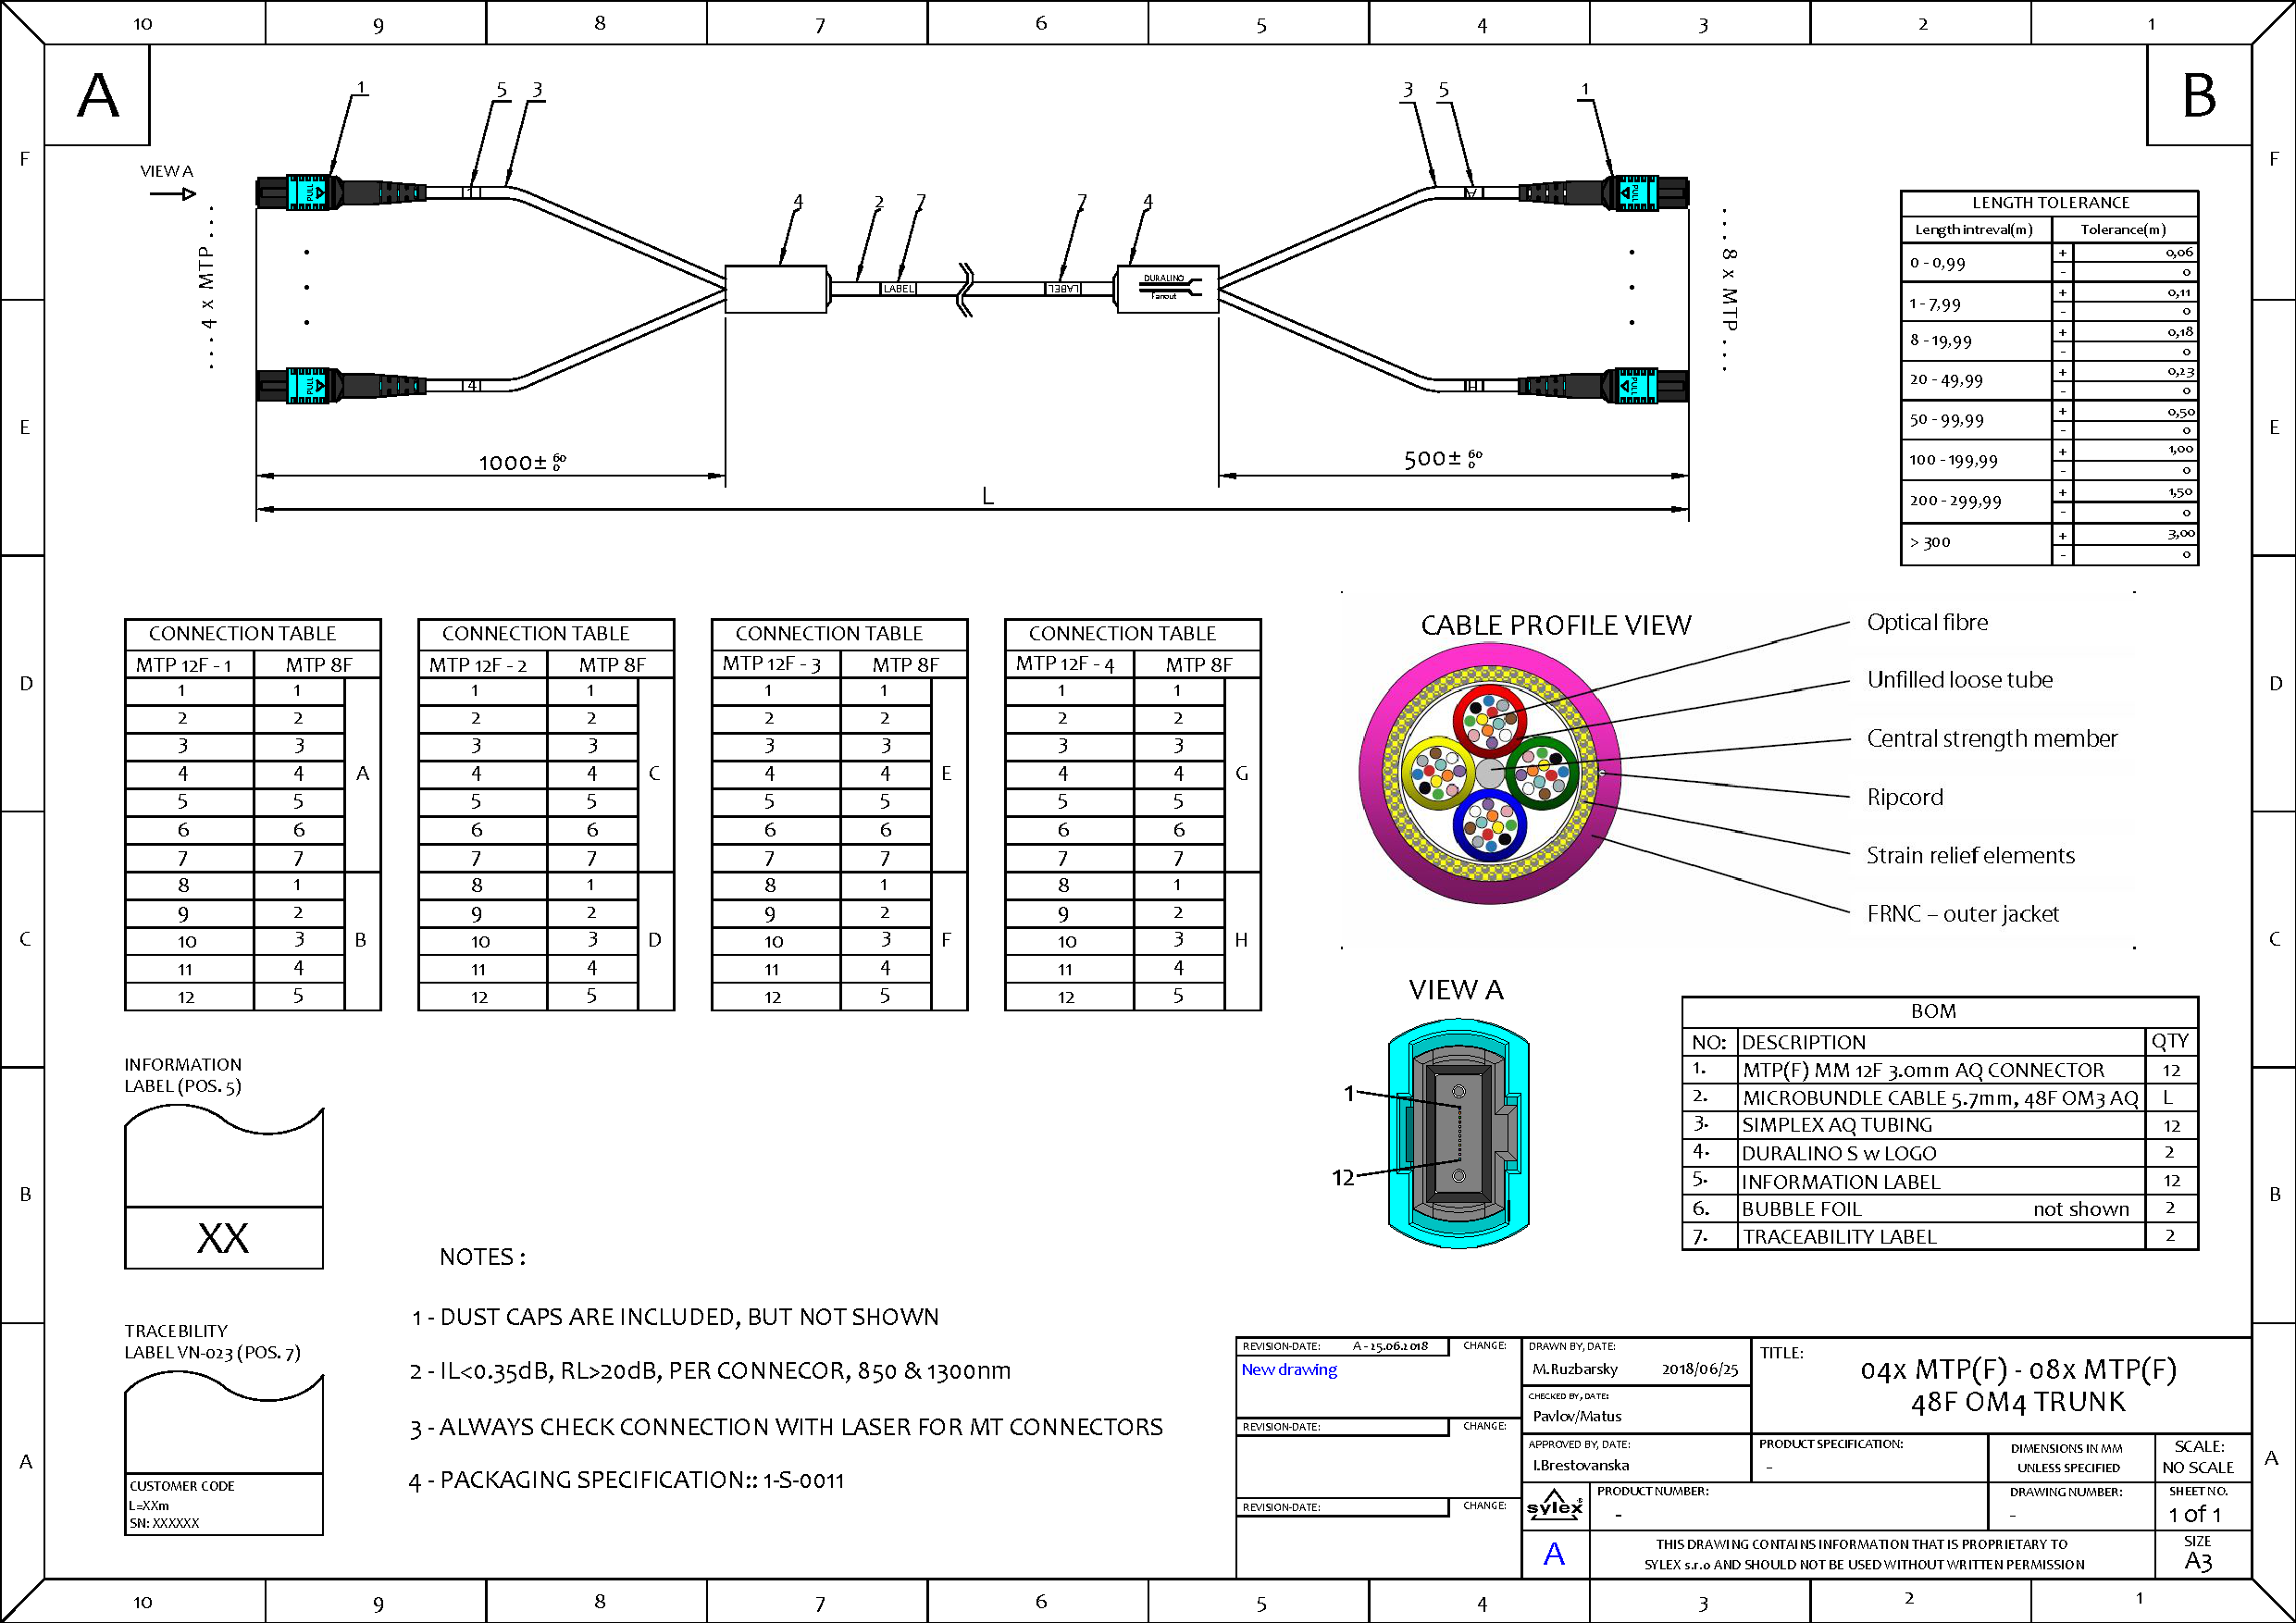
\includegraphics[width=1\textwidth]{Images/Phase2Upgrades/OpticalFibers/TRUNK_C2202.pdf}
    \caption{A technical diagram and manufacturer's specifications for a 48-fiber bundle trunk.}
    \label{fig:trunkspecs}
\end{figure}

\begin{figure}[H]
    \centering
    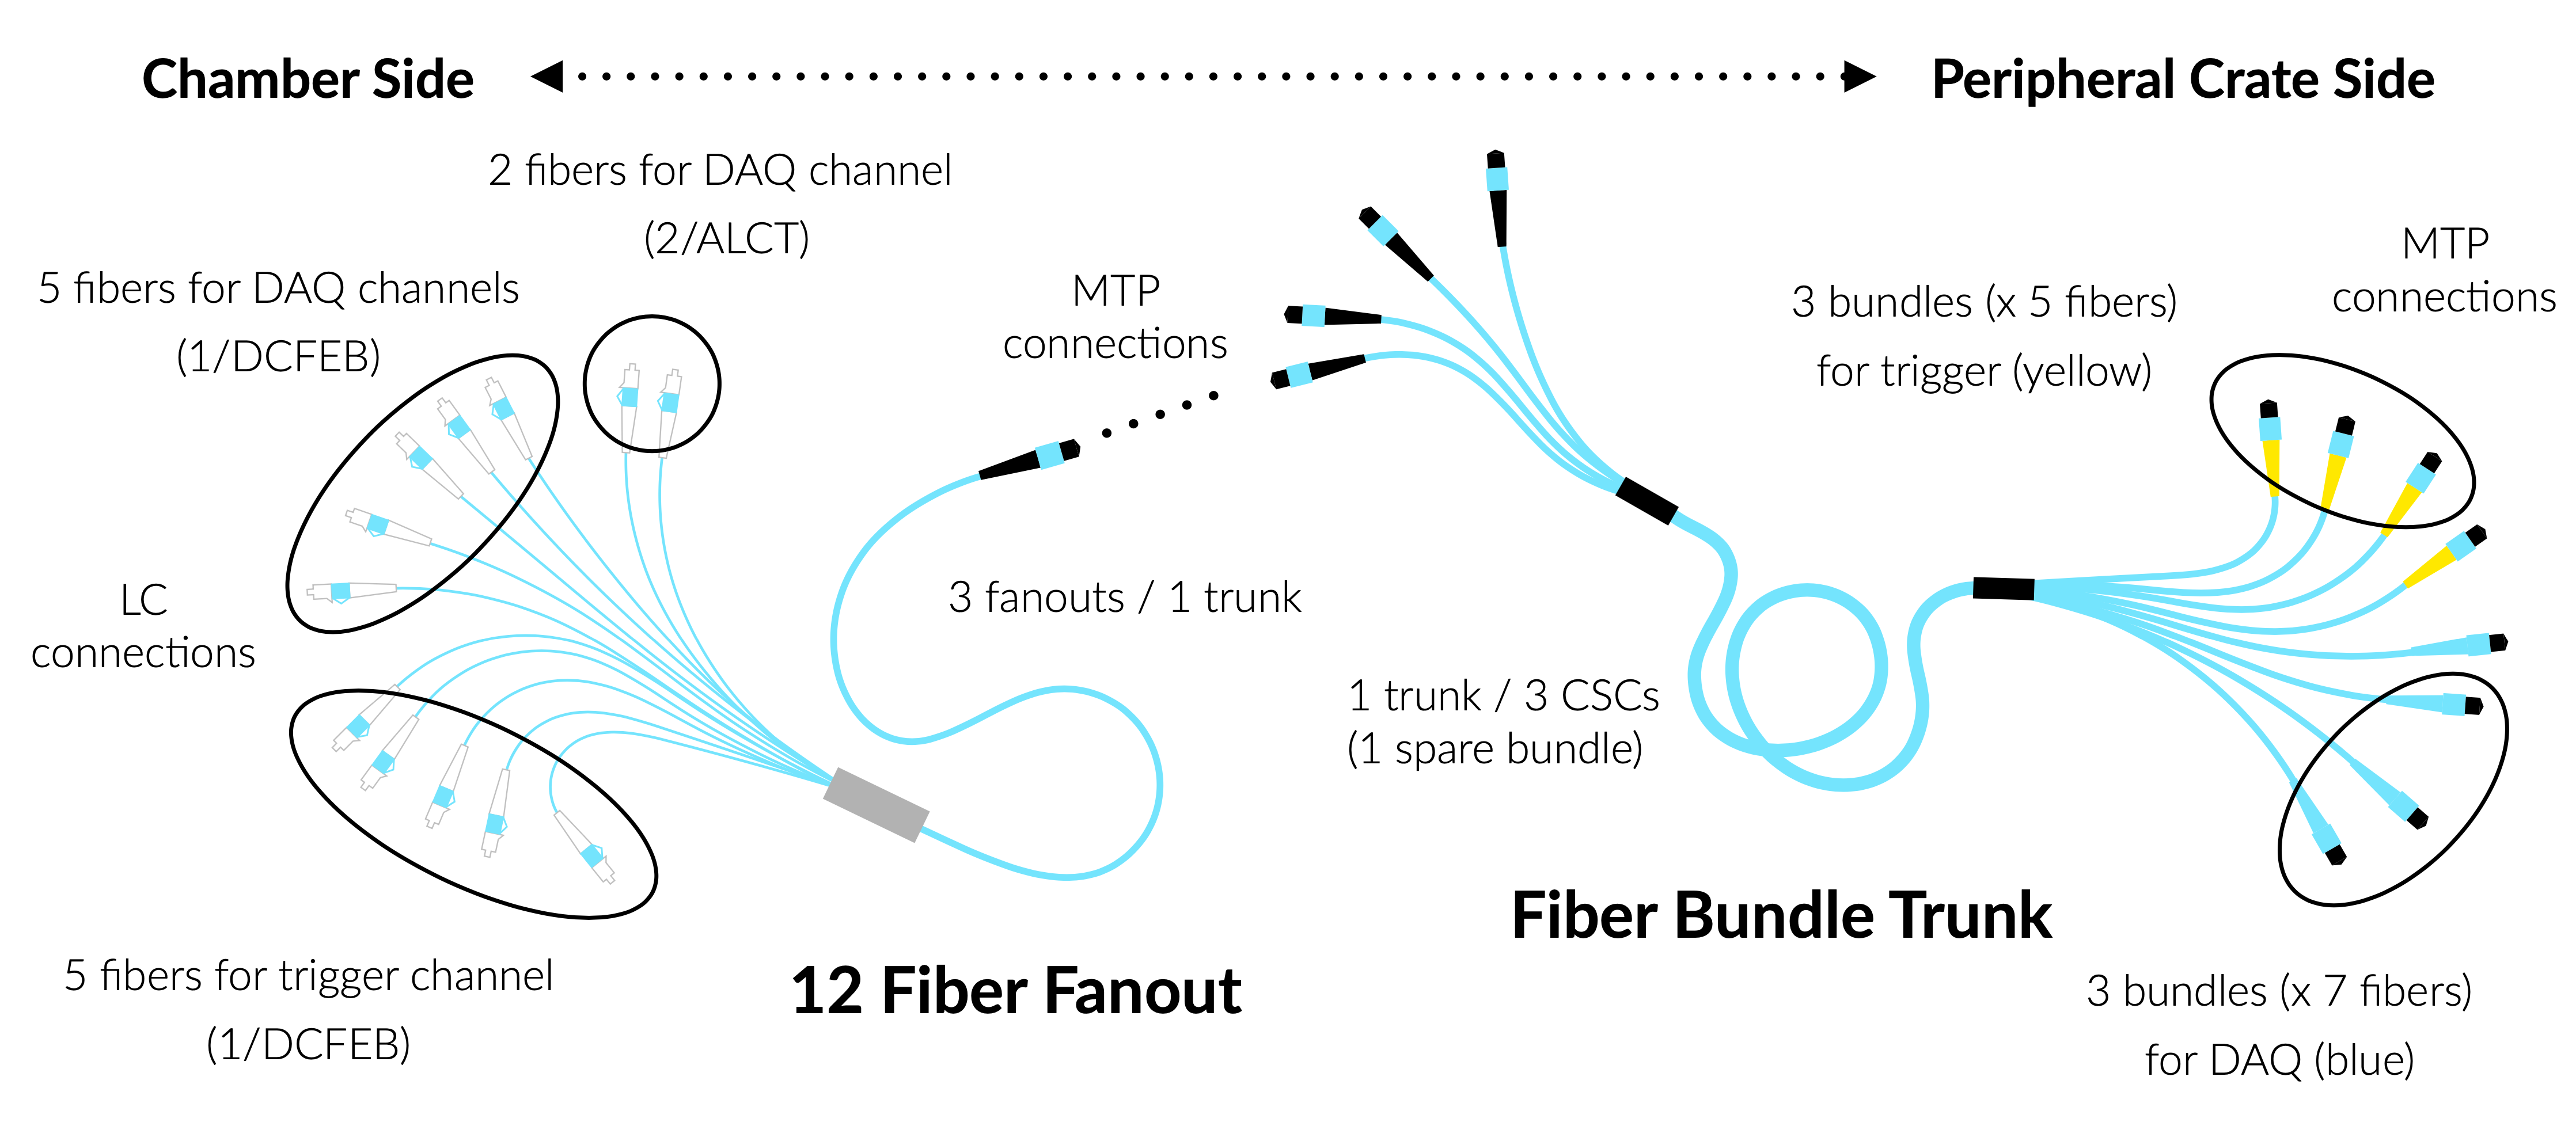
\includegraphics[width=1\textwidth]{Images/Phase2Upgrades/OpticalFibers/FanoutTrunkCartoon.png}
    \caption{A cartoon diagram depicting the fanout-to-trunk setup for three CSCs, from chamber to peripheral crate.}
    \label{fig:fanouttrunkcartoon}
\end{figure}

Functionality and mapping of the 48-fiber bundle trunks were tested in building 904 at the CERN Prevessin site. The testing setup consisted of an ME1/1 chamber, who's DCFEB acted as a constant light source. The LC ends of a 12-fiber fanout were connected to the DCFEB and the MTP end was connected to fiber bundles 1-4. The other end of the trunk, bundles A-H, were also connected to the MTP end of a second fiber fanout, and the LC connectors of those were connected to an attenuation meter. By observing light in all 48 fibers channel, one by one, the mapping of each fiber on the four-bundle-split to the eight-bindle-split of the trunk was validated. Optical attenuation measurements were consistent accross channels and within the manufacturer's specifications, shown in Fig.. At the CSC facility in SX5, mapping and attenuation of ten 12-fiber fanouts were studied, using a setup similar to the one used in bulding 904, the difference being the 48 fiber bundle trunk was replaced with a single 12-fiber bundle trunk with just one MTP connection on each end. A photograph of the SX5 setup is provided in Fig.~\ref{fig:fibertestsetup}. Optical attenuation measurements made for each of the ten 12-fiber fanouts can be found in Fig.~\ref{fig:fanoutattenuation}.

\begin{figure}[H]
    \centering
    \includegraphics[width=0.49\textwidth]{Images/Phase2Upgrades/OpticalFibers/FanoutTesting.png}
    \caption{The 12-fiber fanout testing setup at the CSC facility in SX5. The LC-ends of a fanout were connected to the Finnesar links on right-most DCFEB (obscured by a cooling cover). On the table in the foreground is one of the 12-fiber fanouts being tested, connnected to the the 12-fiber trunk and the optical attenuation meter.}
    \label{fig:fibertestsetup}
\end{figure}

\begin{figure}[H]
    \centering
    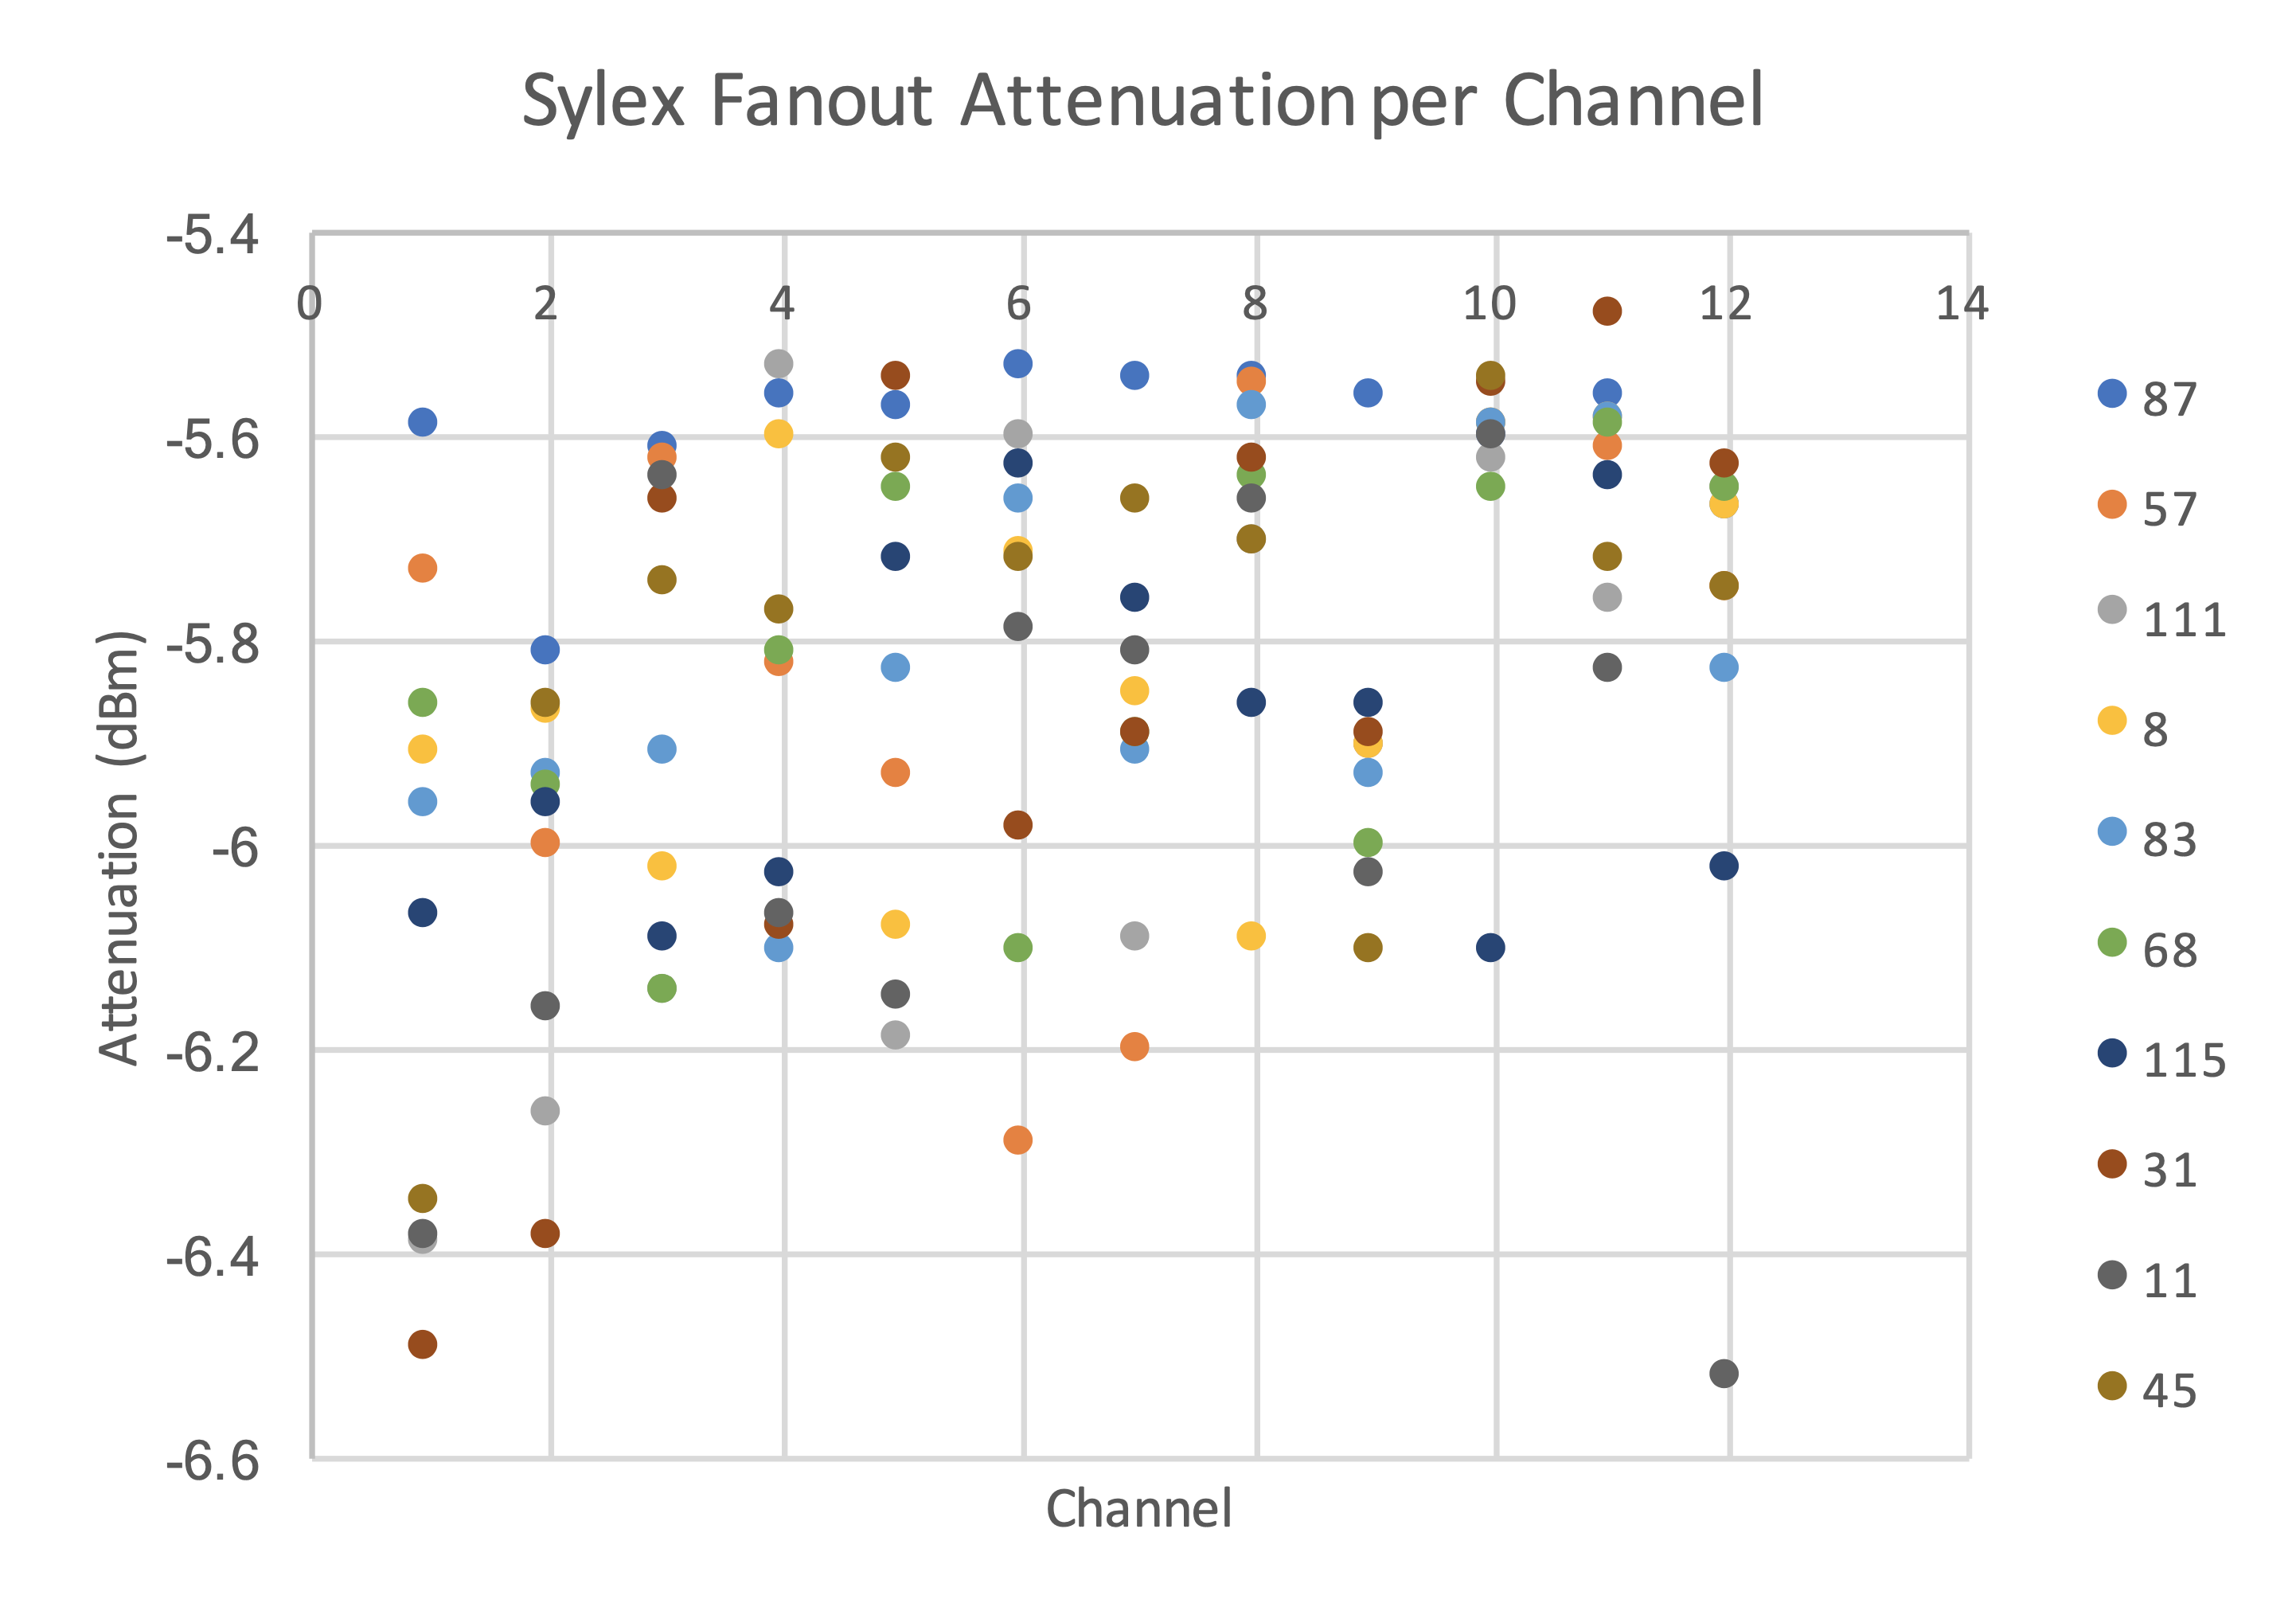
\includegraphics[width=0.75\textwidth]{Images/Phase2Upgrades/OpticalFibers/FanoutAttenuation.png}
    \caption{Optical attenuation in each channel of ten 12-fiber fanouts. Each color corresponds to a different fanout.}
    \label{fig:fanoutattenuation}
\end{figure}

Routing of the thirty-six 48-fiber bundle trunks was performed during LS2 when access to CSC stations 1, 2, and 3 was possible. As the orientation of chambers in stations alternate in each endcap, two routing configurations were used, shown in Fig.~\ref{fig:fiberrouting}. Fiber bundle trunks were secured to the sides of ME234/2 chambers with sticky pads and cable ties (the procedure is demonstrated in the two photographs of Fig.~\ref{fig:MishaGabrielRoutingFibers}), while the MTP ends on the rack-side of the trunk were bound together and wrapped in a platic bag. During LS3, the fiber bundles will be connected to each chamber and to the OTMB and ODMB in the peripheral racks. Prior to routing, labels were applied to all the trunks: two on the middle trunk near the two splits, and one near the MTP connector on each bundle. Chamber-side bundles were labeled with either the chamber (e.g., ``ME-1/1/1'') or ``SPARE,'' while crate-side bundles were labeled with the rack/crate/slot numbers, chamber, and either TRG or DAQ, depending on if the bundle was for trigger or data channels. The middle of the trunks were labeled with the chamber range/TRG+DAQ/rack/crate and a barcode.

\begin{figure}[H]
    \centering
    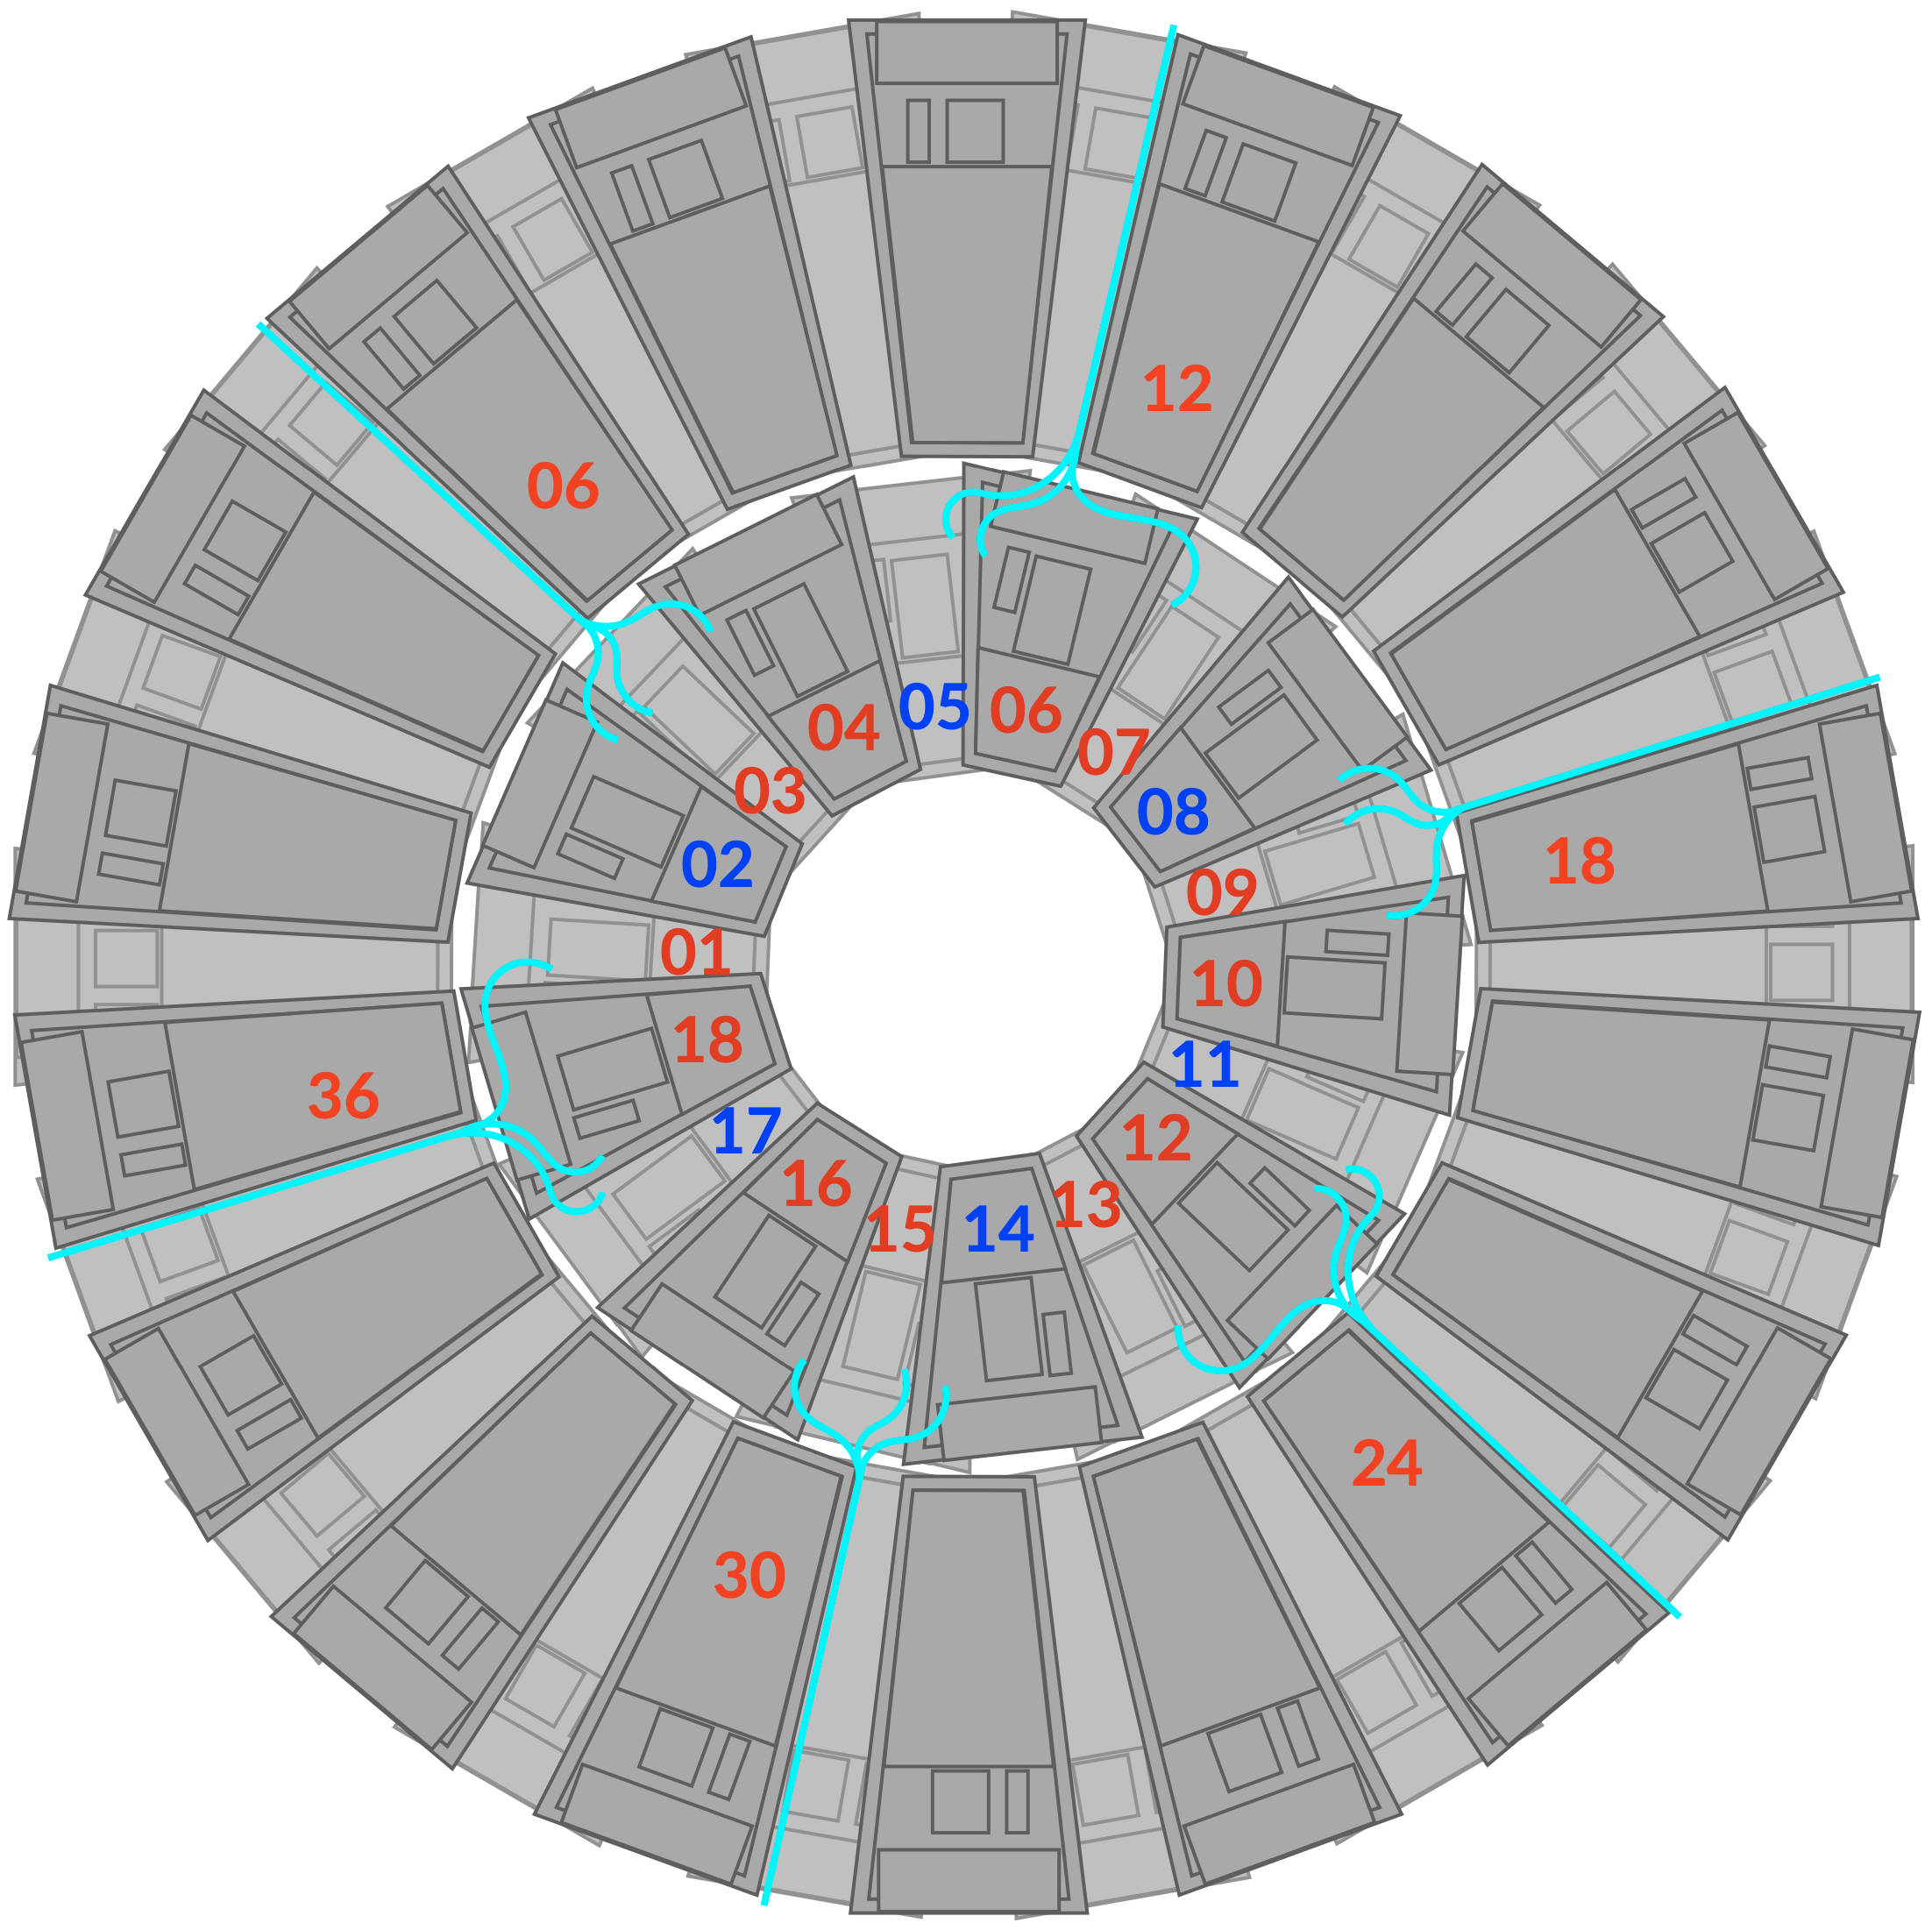
\includegraphics[width=0.49\textwidth]{Images/Phase2Upgrades/OpticalFibers/FiberRouting1.png}
    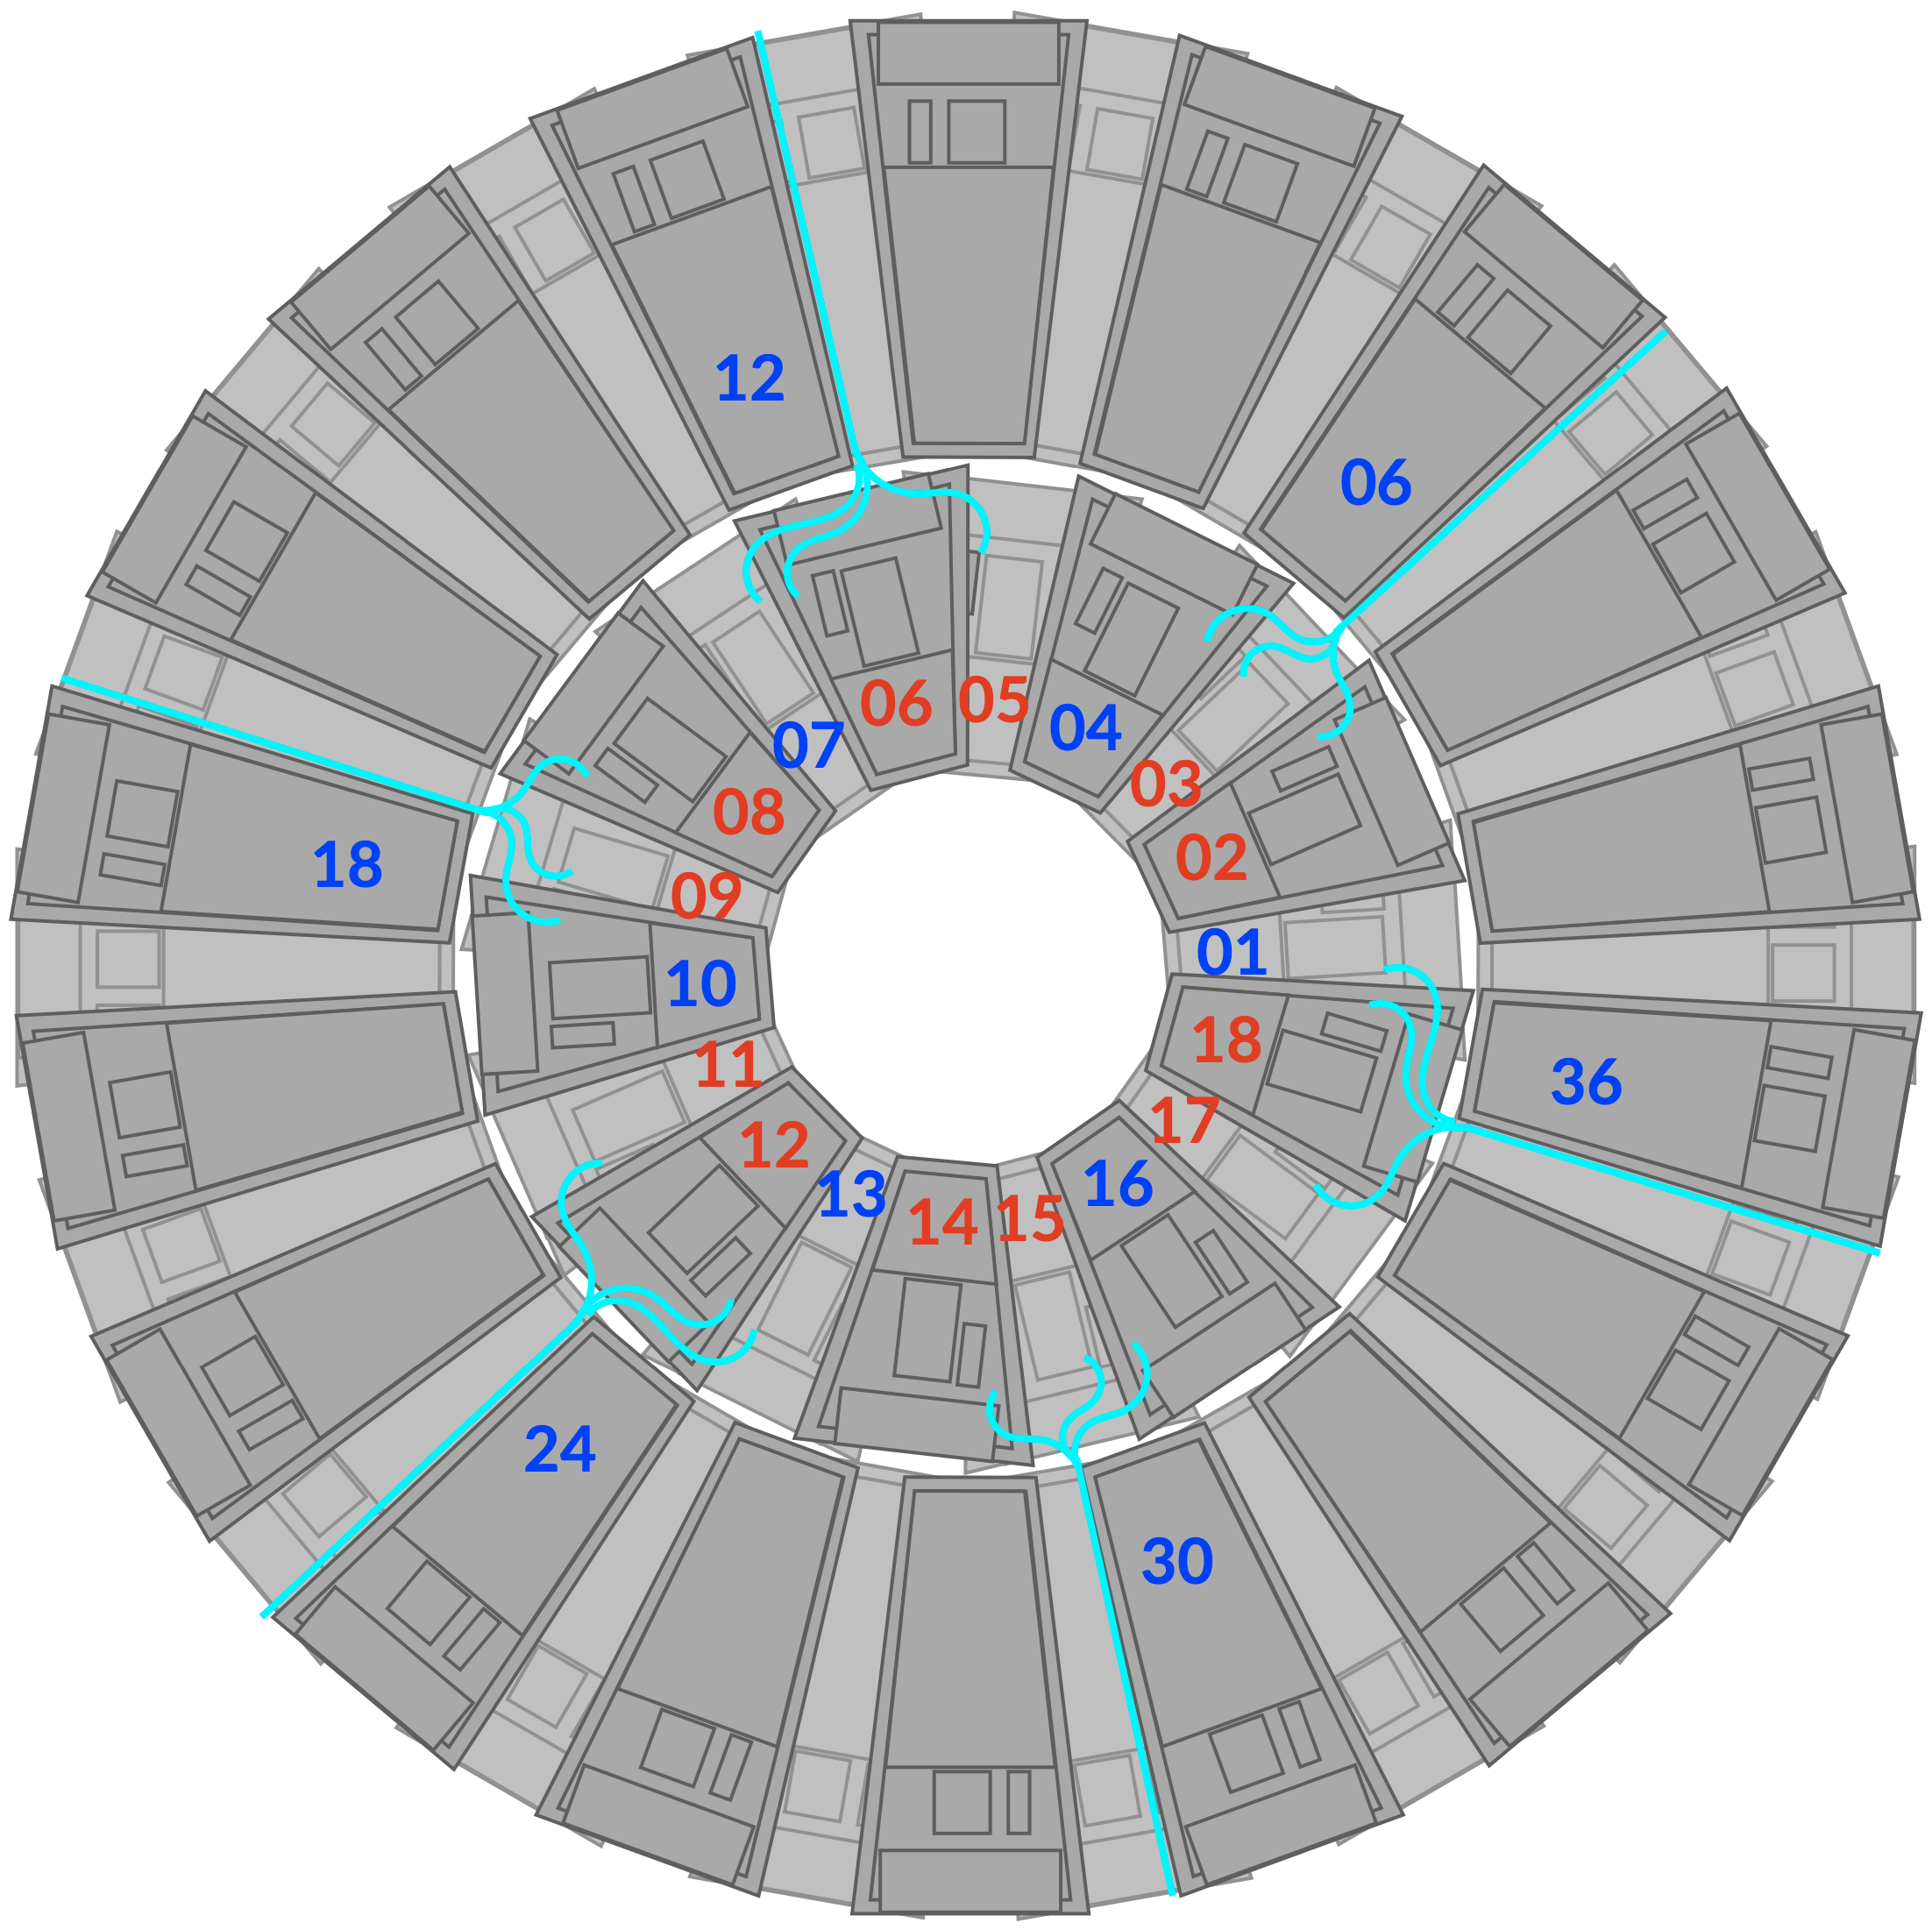
\includegraphics[width=0.49\textwidth]{Images/Phase2Upgrades/OpticalFibers/FiberRouting2.png}
    \caption{A schematic of the 48-fiber bundle trunk routing configurations on different endcap disks. Left: Fiber routing for clockwise-oriented stations, ME+2, ME-3, and ME-4. Right: Fiber routing for counter-clockwise-oriented stations, ME-2, ME+3, and ME+4. Chambers where the fiber bundle/trunk is connected/secured to the HV side are labeled in red, while chambers where the fiber bundle/trunk is connected/secured to the non-HV side are labeled in red.}
    \label{fig:fiberrouting}
\end{figure}

\begin{figure}[H]
    \centering
    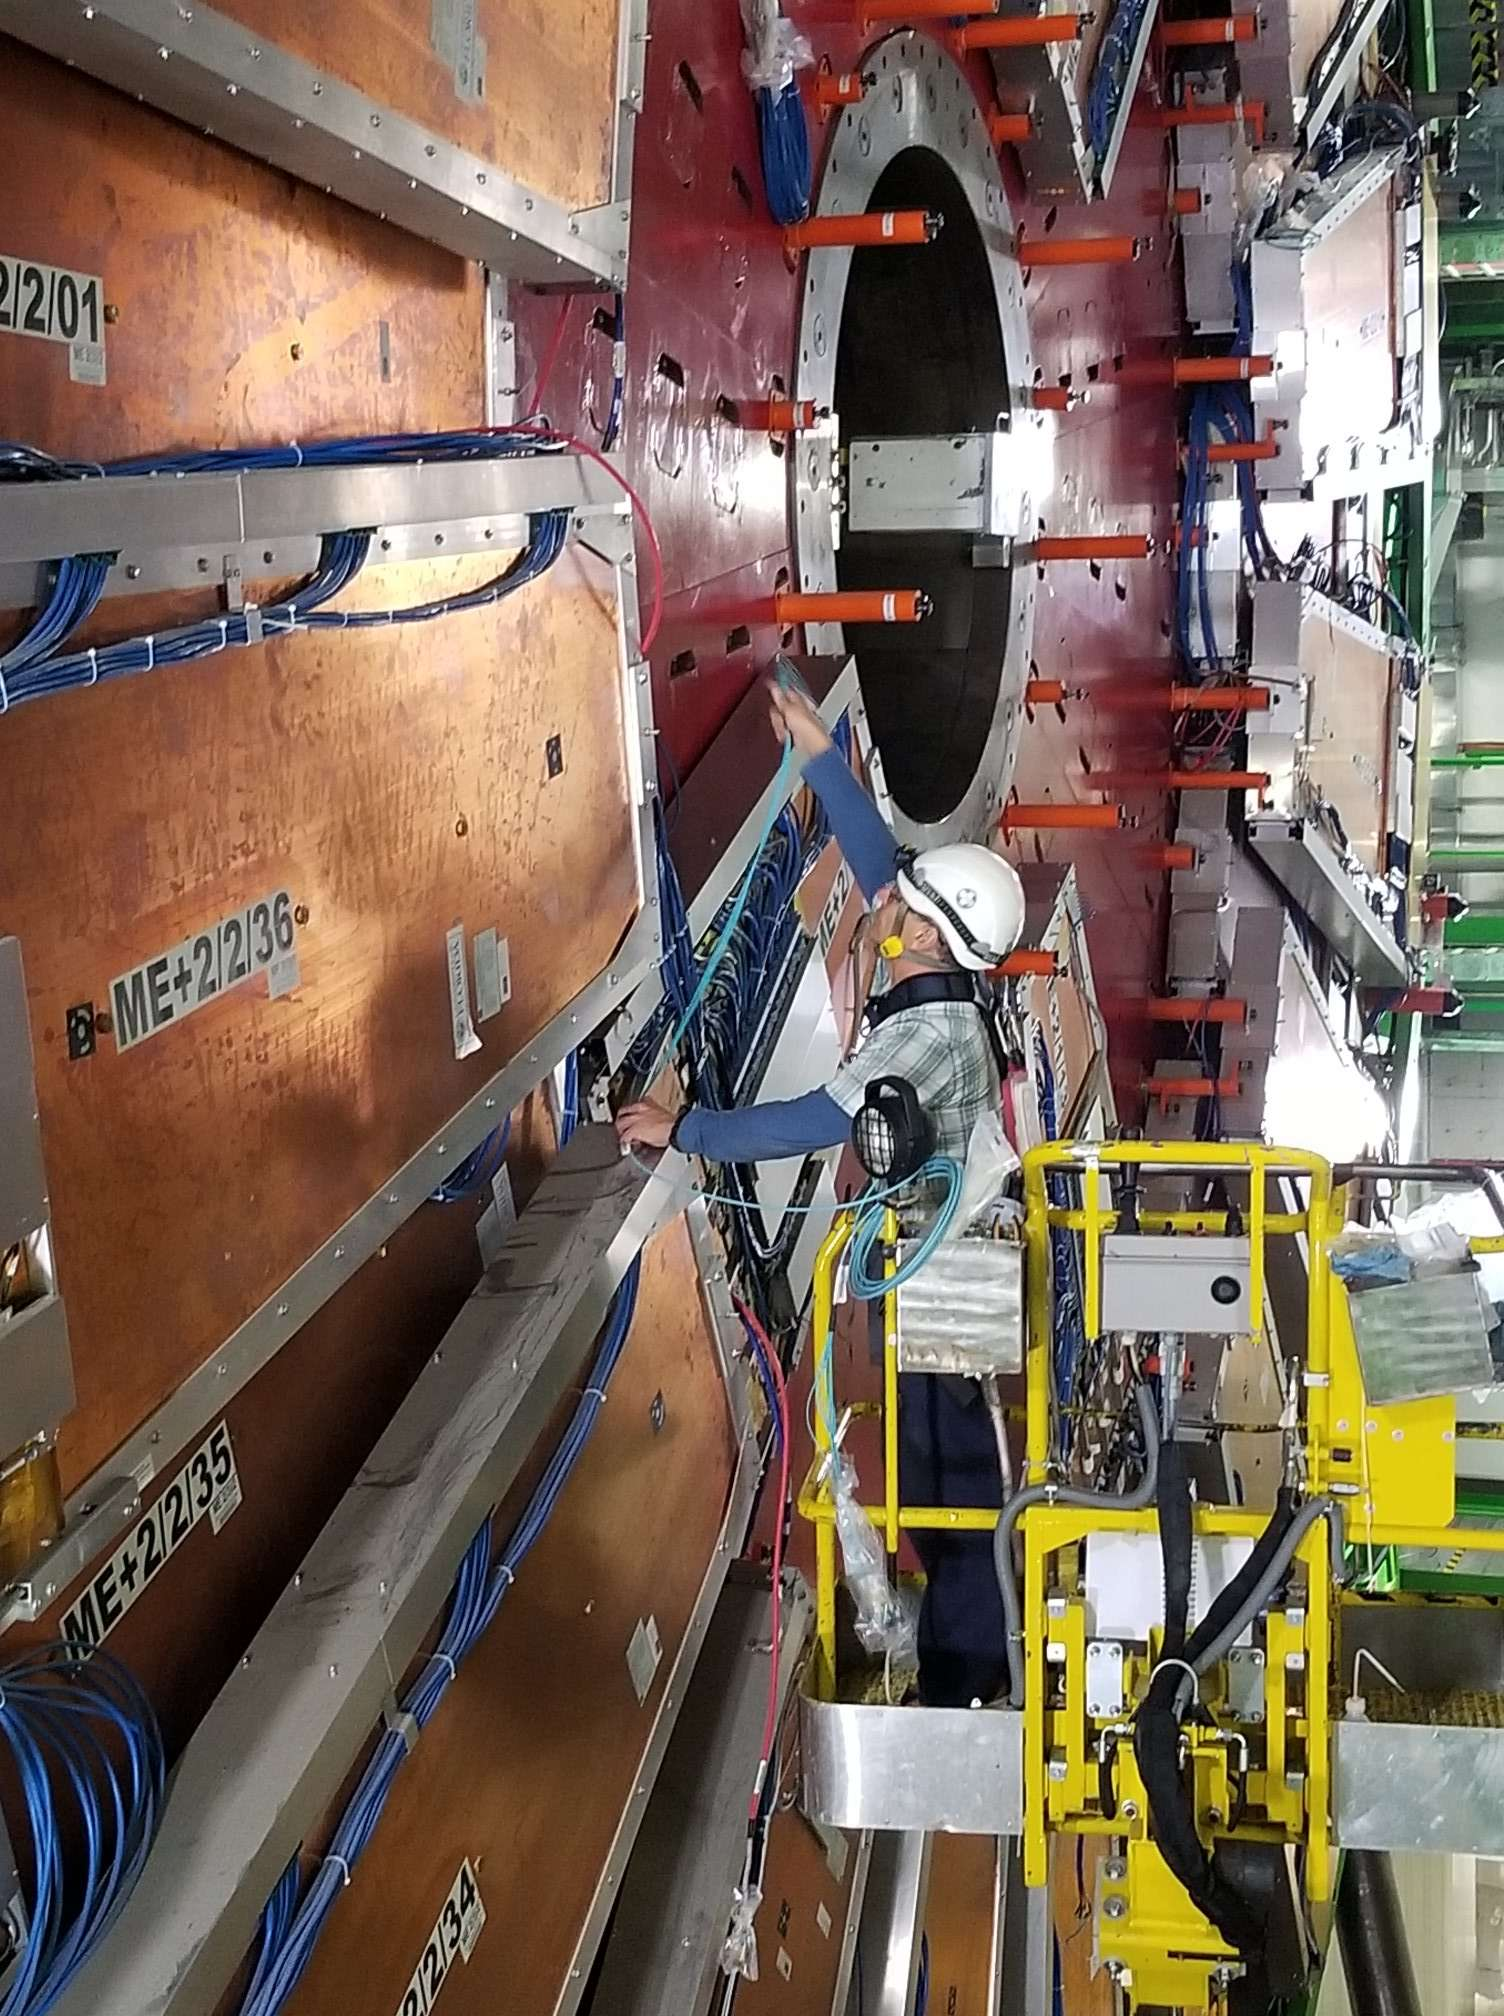
\includegraphics[width=0.49\textwidth]{Images/Phase2Upgrades/OpticalFibers/MishaRoutingFibers.jpeg}
    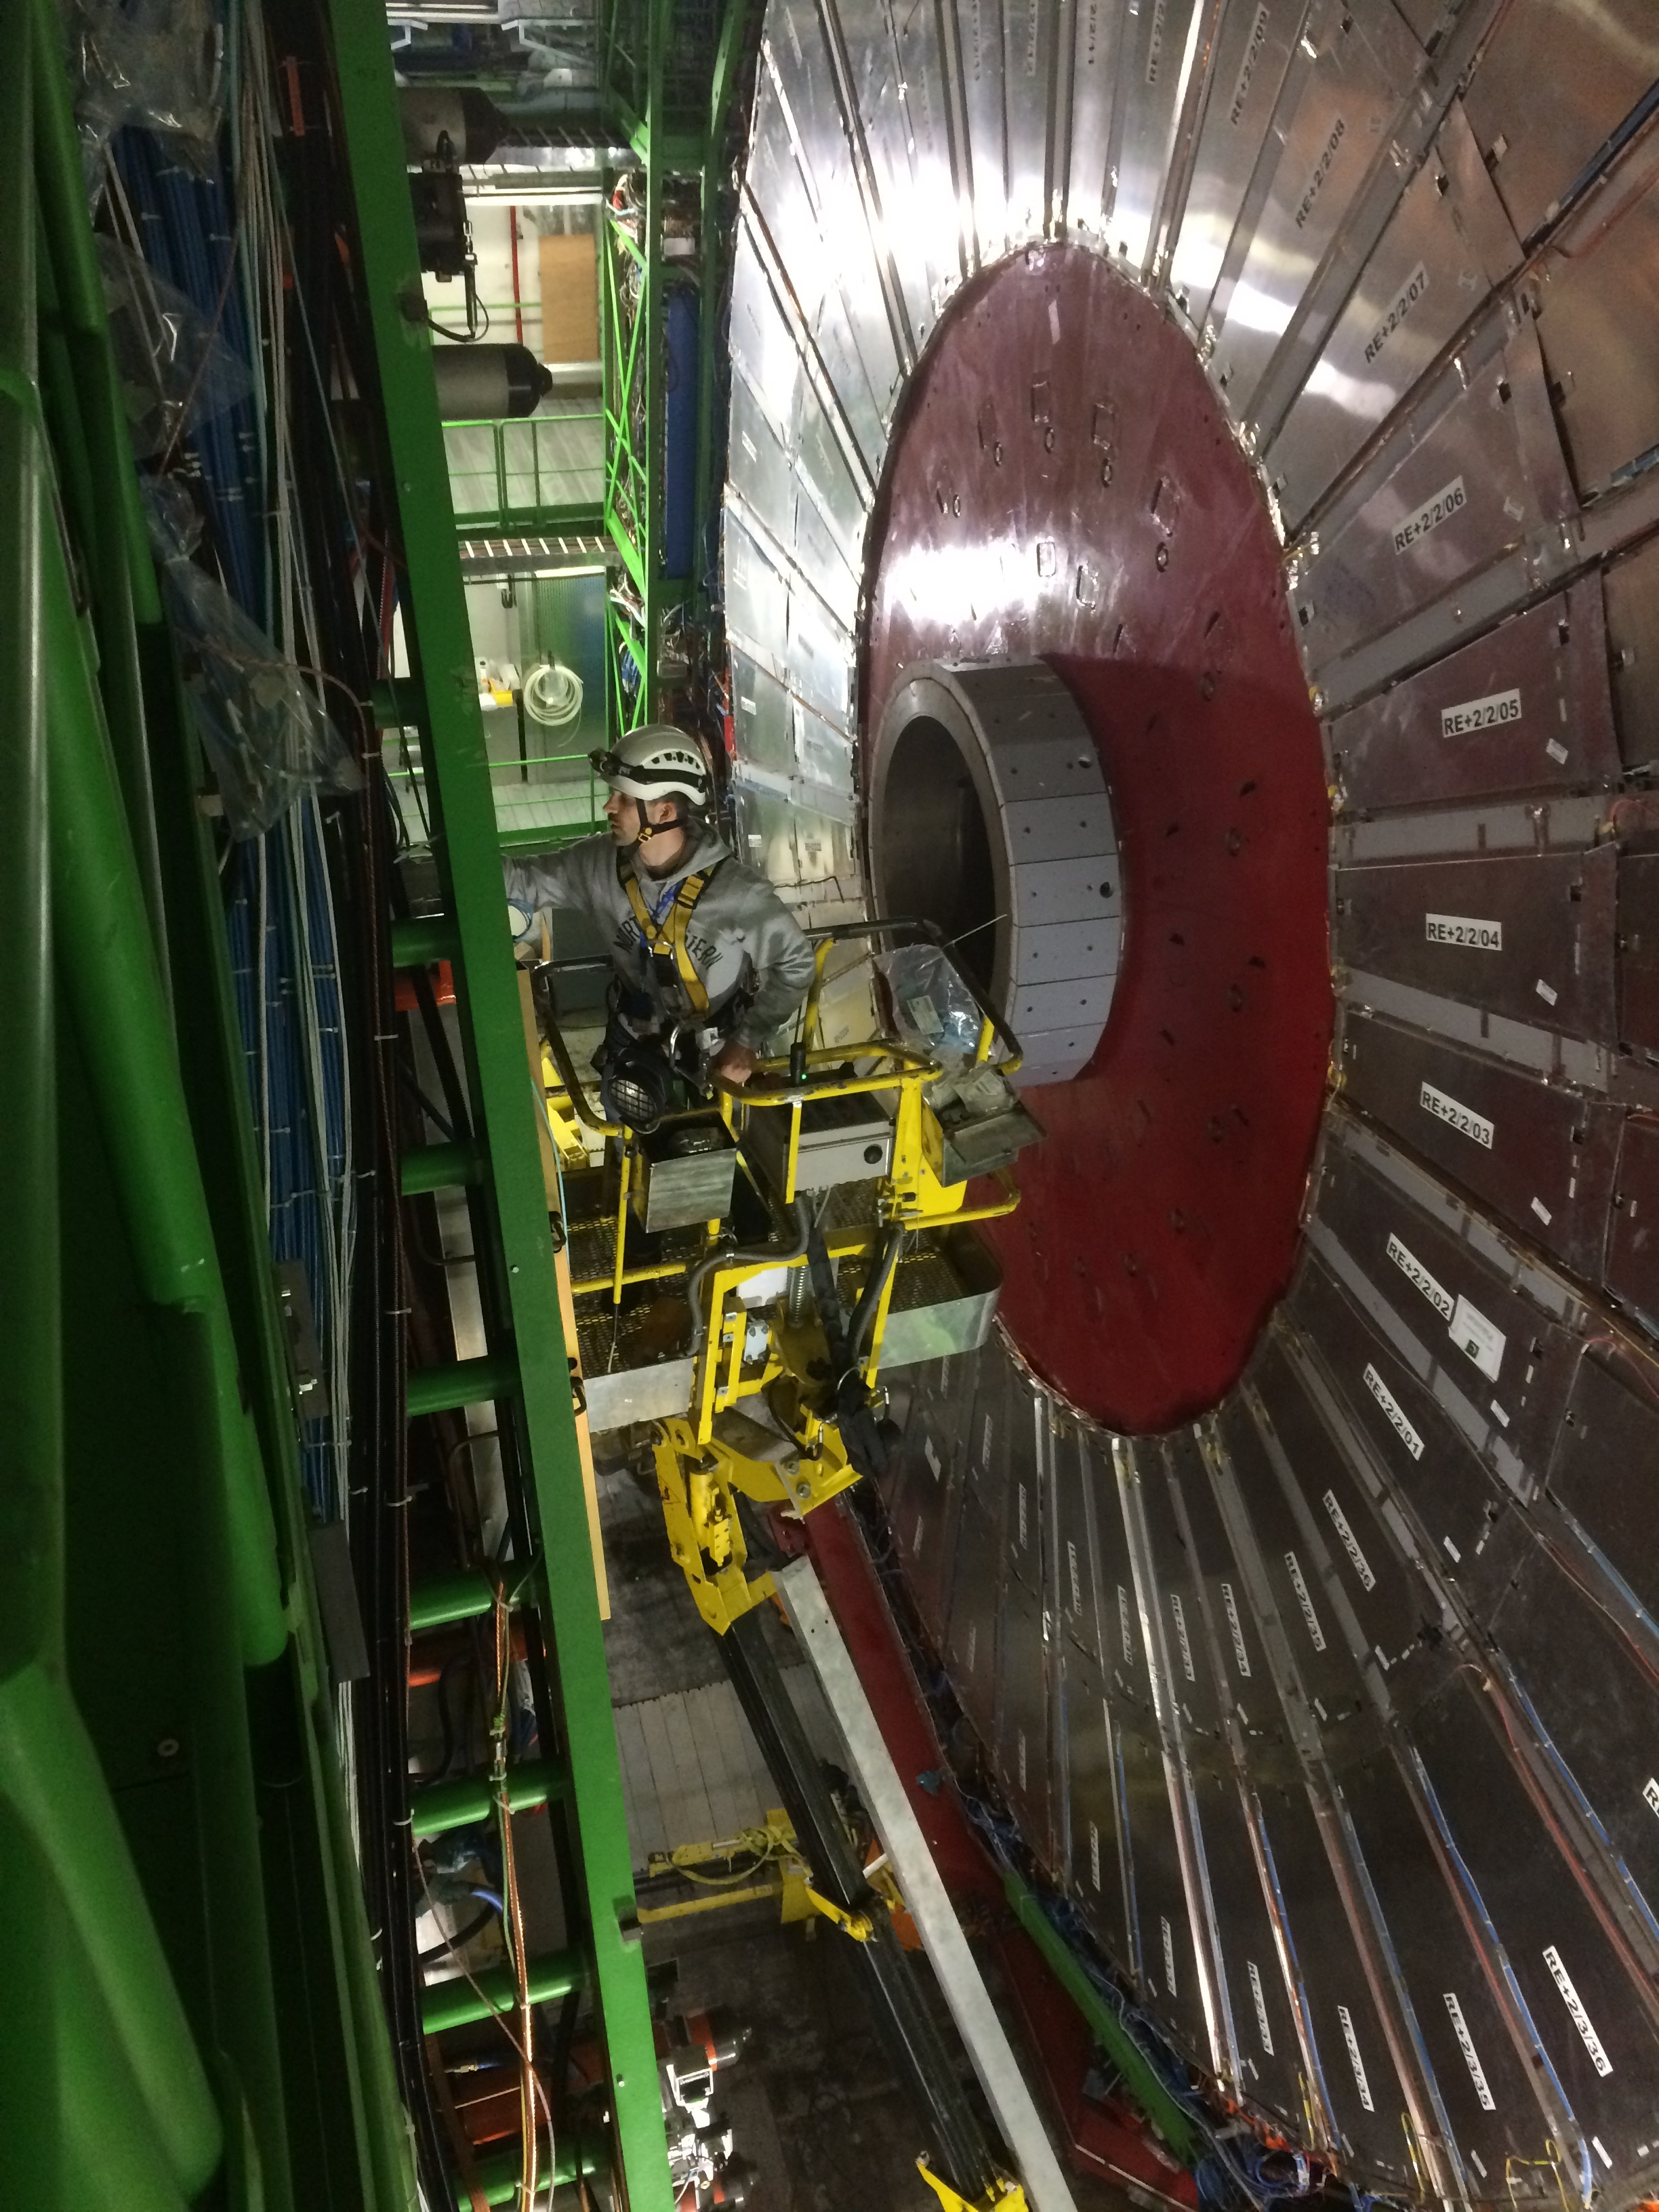
\includegraphics[width=0.49\textwidth,angle=270]{Images/Phase2Upgrades/OpticalFibers/GabrielRoutingFibers.jpg}
    \caption{Routing of the 48-fiber bundle trunks on the ME+2 disk by Misha Ignatenko (left) and the author (right).}
    \label{fig:MishaGabrielRoutingFibers}
\end{figure}